\section{实验:用电磁继电器控制电路}\label{sec:10-7}

在这个实验里,我们练习使用电磁继电器。图 \ref{fig:10-31} 是利用电磁继电器来控制小电动机的电路。
仔细观察电磁继电器的构造,分析它在通、断电时触点的闭合情况。
然后根据电路图,想清楚控制电路中的电键 $K$ 闭合或断开时,工作电路里哪个支路中的小电动机转动。

\begin{figure}[htbp]
    \centering
    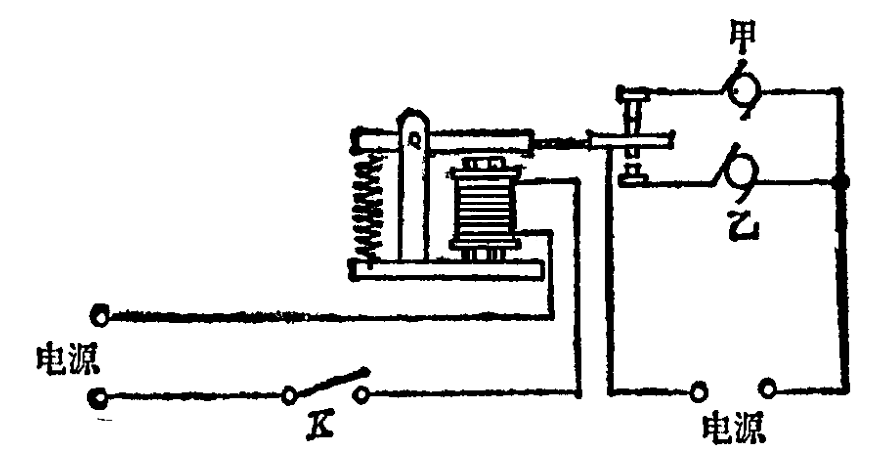
\includegraphics[width=0.6\textwidth]{../pic/czwl2-ch10-31}
    \caption{}\label{fig:10-31}
\end{figure}

实验时按照图 \ref{fig:10-31} 连接电路,先把小电动机连接在甲支路中,乙支路暂不连接,
观察当电键 $K$ 闭合或断开时,继电器对小电动机的控制情况。
再把小电动机换接在乙支路中,甲支路暂不连接,
观察当电键 $K$ 闭合或断开时,继电器对小电动机的控制情况。
最后把两个小电动机分别连接在甲、乙两个支路中,
观察当电键 $K$ 闭合或断开时,继电器对两个小电动机的控制情况。

这个实验也可以用小灯泡代替小电动机来做。



\lianxi

(1) 电磁铁的磁性强弱是由什么决定的?设计一个磁性强弱可以改变的电磁铁,画出它的电路图。


(2) 图 \ref{fig:10-32} 是一种防汛报警器的原理图。 $K$ 是触点开关,
$B$ 是一个漏斗形的竹片圆筒,里面有个浮子 $A$。试说明这种报警器的工作原理。

\begin{figure}[htbp]
    \centering
    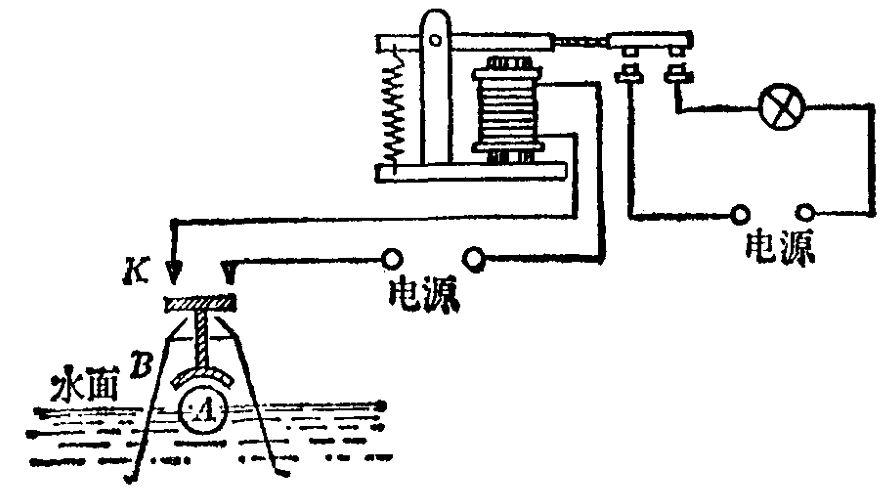
\includegraphics[width=0.6\textwidth]{../pic/czwl2-ch10-32}
    \caption{}\label{fig:10-32}
\end{figure}

(3) 在图 \ref{fig:10-33} 所示的装置中,当工作电路发生故障而断开的时候,指示灯就发光告警;
故障排除后工作电路接通,指示灯就熄灭。为什么?

\begin{figure}[H]%[htbp]
    \centering
    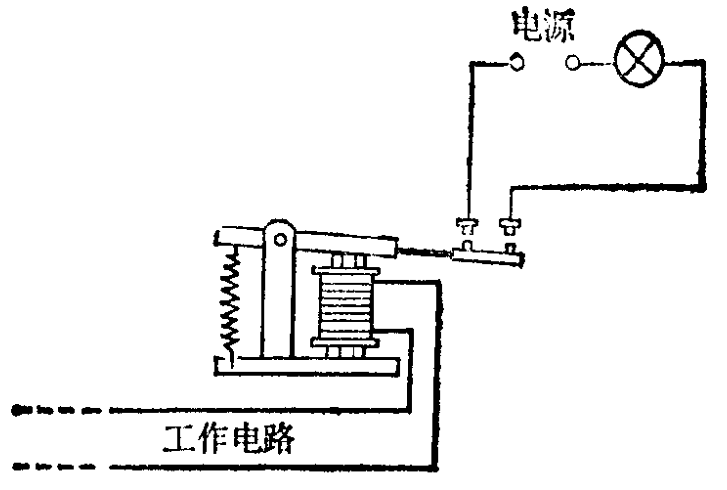
\includegraphics[width=0.6\textwidth]{../pic/czwl2-ch10-33}
    \caption{}\label{fig:10-33}
\end{figure}

(4) 图 \ref{fig:10-34} 是一种水位自动报警器的原理图。
水位没有达到金属块 $B$ 时,绿灯亮;水位达到金属块 $B$ 时,红灯亮。
试说明它的工作原理。注意:纯净的水不导电,但一般的水都是导电的。

\begin{figure}[htbp]
    \centering
    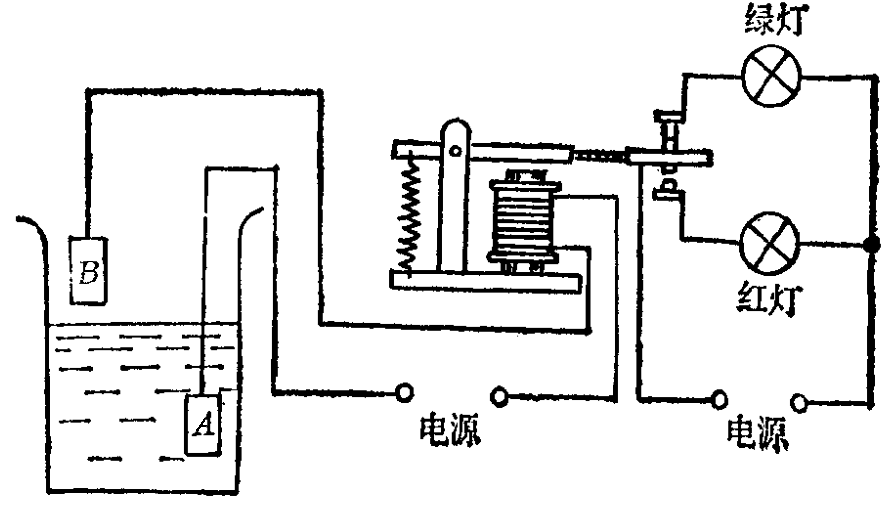
\includegraphics[width=0.6\textwidth]{../pic/czwl2-ch10-34}
    \caption{水位自动报警器的原理}\label{fig:10-34}
\end{figure}

(5) 图 \ref{fig:10-35} 是一种温度自动报警器的原理图,图中 1 是电磁铁,
2 是弹簧片,3 是触点,4 是水银温度计,在水银温度计的管里封入一段金属丝。
当温度达到金属丝下端所指的温度时,电铃就响起来,发出报警信号。 试说明它的原理。

\begin{figure}[htbp]
    \centering
    \begin{minipage}{7cm}
    \centering
    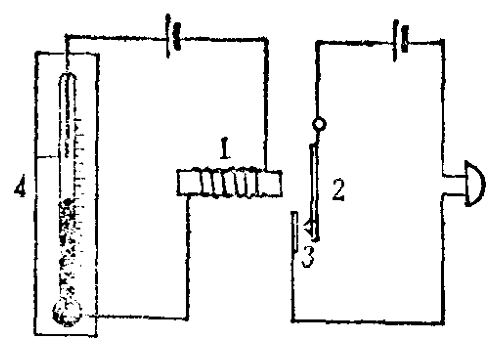
\includegraphics[width=7cm]{../pic/czwl2-ch10-35}
    \caption{温度自动报警器的原理}\label{fig:10-35}
    \end{minipage}
    \qquad
    \begin{minipage}{7cm}
    \centering
    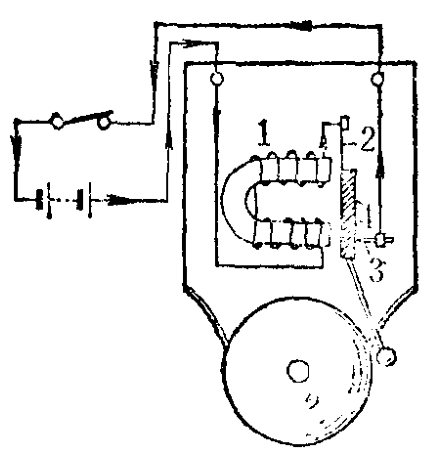
\includegraphics[width=6cm]{../pic/czwl2-ch10-36}
    \caption{}\label{fig:10-36}
    \end{minipage}
\end{figure}

\section*{小实验}

你们都见过电铃吧!电铃也是利用电磁铁来工作的。下面简单介绍一下电铃的构造,
你们可以根据这个介绍自己寻找合适的材料自制一个电铃,看谁做的最好。

电铃的构造如图 \ref{fig:10-36} 所示。
1 是电磁铁, 2 是弹簧片, 3 是螺钉, 4 是衔铁,衔铁与螺钉的尖端紧靠着。
当按下电键的时候,电路接通,电磁铁有了磁性,把弹簧片上的衔铁吸过来,弹簧片下端的小锤就在铃上打一下。
当衔铁被吸过来时,它和螺钉尖端分开,电路被切断,电磁铁立即失去磁性,弹簧片便弹了回去。
衔铁一接触螺钉,电路又通了,又把衔铁吸过来,小锤又敲击铃,铃又响了一下。
只要电键合着,电流就这样一断一通地循环下去,铃声也就响个不停。

你的电铃做好以后,接上电源,闭合开关,电铃到底响不响?
假如不响,你不要灰心,要仔细检查改进,只要你耐心并善于利用你的知识,你终究会把它弄响的。
我们猜想,当你自制的电铃响个不停的时候,你一定会满足地笑了起来。

